% Provenance (never printed): enseignement scientifique premiere (2019),
% "La Terre, un astre singulier" (the place of the Earth) and the old seconde
% SVT "La planete Terre, une planete habitable" (conditions for liquid water,
% the habitable zone); see sources/book2/PROVENANCE.md. Every temperature,
% phase boundary and habitable-zone limit is computed in
% figdata/grade-10/planet_temperatures.py.
\chapter{Une planète habitable}\label{ch:g10:habitable-planet}

Trois planètes rocheuses tournent côte à côte autour du Soleil. À la surface
de Vénus, l'air est si dense qu'il presse quatre-vingt-douze fois plus fort
que sur la Terre, et si chaud --- plus de \qty{460}{\degreeCelsius} --- que
le plomb y fondrait. Sur Mars, l'air ténu presse moins d'un centième aussi
fort que le nôtre, et la température moyenne est très inférieure au point de
congélation. Entre les deux, la Terre a des océans, de la pluie et la vie.
Les trois planètes se sont formées dans le même disque de gaz et de
poussières autour du jeune Soleil, à partir de roches à peu près
semblables. Pourquoi des destins si différents~? Ce chapitre examine ce qui
fixe la température d'une planète, ce qui lui permet de garder une
atmosphère, dans quelles conditions l'eau peut être liquide, et où, autour
du Soleil et autour d'autres étoiles, de telles conditions se rencontrent.
% ledger: nasa:venus-atm, nasa:mars-atm, planet:Venus.Tmean

\begin{omfigure}
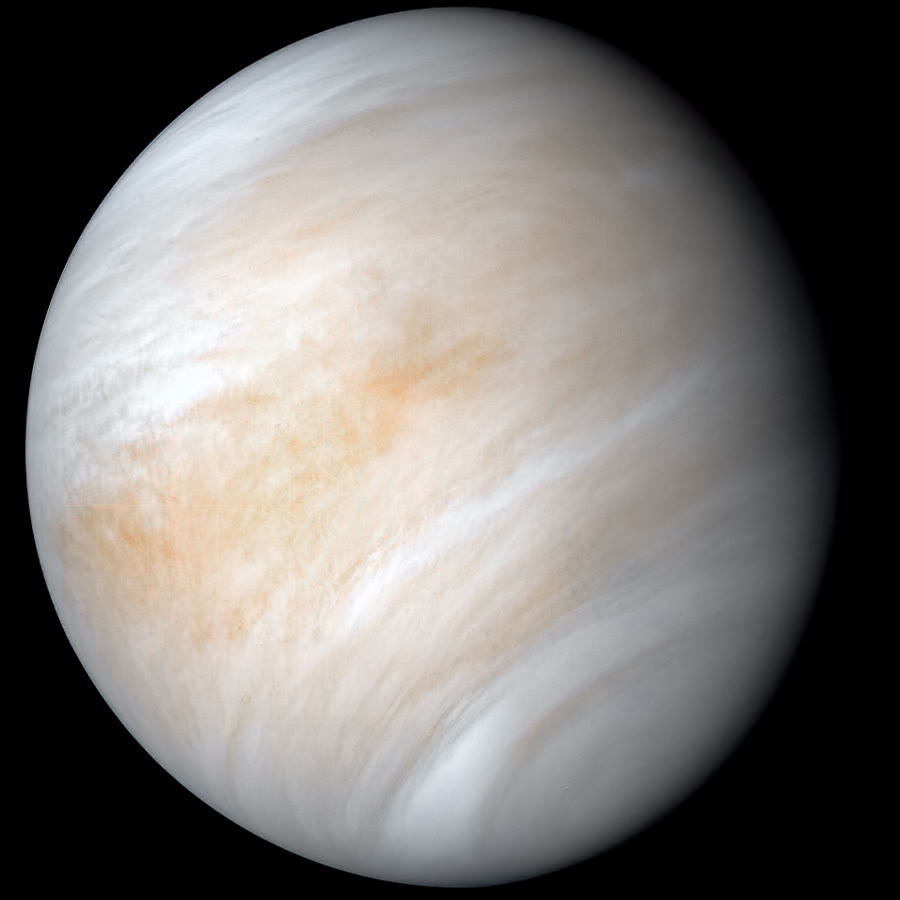
\includegraphics[width=0.38\linewidth]{images/book2/g10-nasa-venus-mariner10.jpg}

{\small Vénus vue par la sonde Mariner~10 en 1974, dans des couleurs proches
de ce que verrait l'œil~: une planète entièrement enveloppée de nuages.
Image~: NASA/JPL-Caltech (domaine public).}
\end{omfigure}

\begin{recall}
Le Soleil est une étoile~; autour de lui, les quatre planètes rocheuses
Mercure, Vénus, la Terre et Mars, puis les quatre planètes géantes,
décrivent des orbites presque circulaires (les livres de physique et le
livre~1). Tout corps rayonne de l'énergie sous forme de lumière, d'autant
plus que sa température est élevée, surtout dans l'infrarouge aux
températures des planètes (les livres de physique). Les gaz à effet de
serre --- vapeur d'eau, dioxyde de carbone, méthane --- absorbent une partie
de l'infrarouge émis par une surface et la maintiennent plus chaude (les
livres de chimie). L'eau existe sous forme de glace, d'eau liquide et de
vapeur d'eau~; la pression est une force par unité de surface, mesurée en
pascals (les livres de physique).
\end{recall}

\section{La température fixée par l'étoile}

Le Soleil envoie sa lumière également dans toutes les directions. À une
distance $d$, sa puissance $L$ (sa \emph{luminosité}) se répartit sur une
sphère d'aire $4\pi d^2$.

\begin{proposition}[La loi en inverse du carré de la lumière solaire]\label{prop:g10:habitable-planet:inverse-square}
La puissance reçue par mètre carré face au Soleil, l'\emph{éclairement
solaire}, à une distance $d$ du Soleil vaut
\[
  S = \frac{L}{4\pi d^2}.
\]
À la distance de la Terre, \qty{1}{au}, $S_0 = \qty{1361}{W/m^2}$~; à une
distance $d$ mesurée en unités astronomiques, $S = S_0/d^2$.
\end{proposition}

\begin{proof}
Aucune lumière ne se perd dans le vide, donc toute la puissance $L$
traverse chaque sphère centrée sur le Soleil~; sur une sphère de rayon $d$,
elle se partage entre $4\pi d^2$ mètres carrés. Doubler $d$ multiplie l'aire
par quatre et divise $S$ par quatre.
\end{proof}
% ledger: earth:TSI, sun:L, const:au

\begin{omfigure}
\begin{tikzpicture}[font=\small, >={Stealth[length=2mm]}]
  \shade[ball color=yellow!70!orange] (0,0) circle (0.35);
  \node[below=4pt] at (0,-0.35) {Soleil};
  \draw[omThm!70, thick] (0,0) -- (3,0.6) (0,0) -- (3,-0.6);
  \draw[omThm!70, thick, dashed] (3,0.6) -- (6,1.2) (3,-0.6) -- (6,-1.2);
  \draw[fill=omDef!25, draw=omDef!80!black] (3,-0.6) rectangle (3.18,0.6);
  \draw[fill=omDef!12, draw=omDef!80!black] (6,-1.2) rectangle (6.18,1.2);
  \draw[omDef!80!black] (6,0) -- (6.18,0) (6.09,-1.2) -- (6.09,1.2);
  \node[anchor=north] at (3.1,-0.7) {$d$};
  \node[anchor=north] at (6.1,-1.3) {$2d$};
  \node[anchor=south east, align=right, font=\footnotesize] at (2.9,0.75) {1 carré~:\\toute la lumière};
  \node[anchor=west, align=left, font=\footnotesize] at (6.35,0.6) {4 carrés~:\\un quart chacun};
  \draw[->, black!60] (0.5,-1.95) -- (6.1,-1.95);
  \node[anchor=north, font=\footnotesize] at (3.3,-2.0) {distance au Soleil};
\end{tikzpicture}

{\small La lumière qui traverse un carré à la distance $d$ se répartit sur
quatre carrés de même taille à la distance $2d$~: l'éclairement décroît
comme l'inverse du carré de la distance.}
\end{omfigure}

Une planète absorbe la partie de cette lumière qu'elle ne réfléchit pas, et
elle rayonne de l'énergie vers l'espace sous forme d'infrarouge. Si elle
absorbe plus qu'elle ne rayonne, elle se réchauffe~; plus chaude, elle
rayonne davantage~; elle se stabilise à la température où les deux
s'équilibrent.

\begin{definition}[Température d'équilibre]\label{def:g10:habitable-planet:equilibrium-temperature}
La \emph{température d'équilibre}\index{temperature d'equilibre@température d'équilibre}
d'une planète est la température à laquelle un corps rayonnant comme un
émetteur parfait enverrait vers l'espace exactement la puissance que la
planète absorbe de son étoile. La fraction de la lumière incidente que la
planète réfléchit dans son ensemble est son \emph{albédo de Bond} $A$.
\end{definition}

\begin{proposition}[Calcul de la température d'équilibre]\label{prop:g10:habitable-planet:teq}
Pour une planète qui répartit la chaleur absorbée sur toute sa surface,
\[
  T_{\mathrm{eq}} = \left(\frac{S\,(1-A)}{4\sigma}\right)^{1/4},
  \qquad \sigma = \qty{5.67e-8}{W.m^{-2}.K^{-4}}.
\]
À la distance de la Terre et sans aucune réflexion, on obtient
\qty{278.3}{K}~; à une distance $d$ en unités astronomiques et avec un
albédo $A$, $T_{\mathrm{eq}} = \qty{278.3}{K} \times (1-A)^{1/4}/\sqrt{d}$.
\end{proposition}

\begin{proof}[Démonstration partielle]
La planète intercepte la lumière solaire sur un disque d'aire $\pi R^2$ et
absorbe la puissance $(1-A)\,S\,\pi R^2$. Elle rayonne par toute sa
surface, $4\pi R^2$. Un émetteur parfait à la température $T$ rayonne
$\sigma T^4$ par mètre carré (une loi démontrée dans les livres de
physique, admise ici). L'égalité $4\pi R^2 \sigma T^4 = (1-A)\,S\,\pi R^2$
donne la formule~; le rayon se simplifie. Avec $S = S_0/d^2$, la racine
quatrième de $1/d^2$ est $1/\sqrt d$.
\end{proof}
% ledger: const:sigma, earth:TSI

\begin{example}[La Terre]\label{ex:g10:habitable-planet:earth}
% ledger: earth:TSI, earth:albedo, earth:Tbb, earth:Tsurf
Avec $S_0 = \qty{1361}{W/m^2}$ et $A = 0.294$,
$T_{\mathrm{eq}} = 278.3 \times 0.706^{1/4} \approx \qty{255}{K}$, soit
\qty{-18}{\degreeCelsius}. (La fiche de la NASA indique \qty{254}{K}.) La
température moyenne de la surface de la Terre est de \qty{288}{K},
\qty{15}{\degreeCelsius}~: l'effet de serre de l'atmosphère la réchauffe
d'environ \qty{33}{K}. Sans lui, les océans gèleraient.
\end{example}

\begin{omfigure}
\begin{tikzpicture}
\begin{axis}[ybar, width=0.86\linewidth, height=5.8cm, ymin=0, ymax=950,
  bar width=10pt, enlarge x limits=0.15, symbolic x coords={Mercury,Venus,Earth,Moon,Mars},
  xtick=data, xticklabels={Mercure,Vénus,Terre,Lune,Mars}, ylabel={température (K)}, ymajorgrids, grid style={gray!22},
  legend style={at={(0.97,0.95)}, anchor=north east, font=\footnotesize, draw=black!30},
  nodes near coords, nodes near coords style={font=\scriptsize, rotate=90, anchor=west, /pgf/number format/fixed, /pgf/number format/precision=0},
  tick label style={font=\small}, label style={font=\small}]
\addplot[fill=omDef!45, draw=omDef!80!black] table[x=name, y=Teq_K] {figdata/out/grade-10-planet_temperatures-planets.dat};
\addlegendentry{température d'équilibre}
\addplot[fill=omThm!55, draw=omThm!80!black] table[x=name, y=Tmean_K] {figdata/out/grade-10-planet_temperatures-planets.dat};
\addlegendentry{température moyenne mesurée à la surface}
\end{axis}
\end{tikzpicture}

{\small \omterm{def:g10:habitable-planet:equilibrium-temperature}{Températures d'équilibre} calculées à partir de la distance et de
l'albédo de Bond de chaque corps, à côté des températures moyennes mesurées
à leur surface. Données~: fiches planétaires de la NASA.}
\end{omfigure}

\begin{remark}[Lire le graphique]\label{rem:g10:habitable-planet:reading}
% ledger: nasa:bond-albedos, planet:Mercury.Tmean, planet:Venus.Tmean, planet:Moon.Tmean, planet:Mars.Tmean, planet:Moon.day, nasa:moon-temps
Pour Mercure et Mars, qui n'ont presque pas d'atmosphère ou une atmosphère
très ténue, la moyenne mesurée est proche de la \omterm{def:g10:habitable-planet:equilibrium-temperature}{température d'équilibre}. La
moyenne de la Lune est inférieure~: ses jours et ses nuits durent chacun
environ deux semaines, et sa surface passe d'environ \qty{95}{K} à
\qty{390}{K}, ce que la formule simple, faite pour une planète qui répartit
sa chaleur uniformément, ne rend pas. Vénus est le cas frappant~: avec un
albédo de Bond de 0.77 --- ses nuages réfléchissent la plus grande partie de
la lumière solaire ---, sa \omterm{def:g10:habitable-planet:equilibrium-temperature}{température d'équilibre} est plus basse que celle
de la Terre, et pourtant sa surface est plus chaude de plus de
\qty{500}{K}~: c'est l'effet de serre de son épaisse atmosphère de dioxyde
de carbone.
\end{remark}

\section{Garder une atmosphère}

Un gaz est fait de molécules en mouvement incessant, d'autant plus rapides
que le gaz est chaud. Une molécule située au sommet d'une atmosphère qui
monte plus vite que la vitesse de libération de la planète --- la vitesse
nécessaire pour échapper définitivement à sa gravité (les livres de
physique) --- est perdue dans l'espace. En des milliards d'années, une
petite planète à la gravité faible perd son air~; une grande le garde.

\begin{center}
\small
% ledger: planet:Mercury.vesc, planet:Venus.vesc, planet:Earth.vesc, planet:Moon.vesc, planet:Mars.vesc, planet:Mercury.psurf, planet:Venus.psurf, planet:Earth.psurf, planet:Moon.psurf, nasa:mars-atm
\begin{tabular}{lccc}
\hline
corps & vitesse de libération (\unit{km/s}) & pression en surface (bar) & atmosphère \\
\hline
Lune & 2.4 & 0 & aucune \\
Mercure & 4.3 & 0 & aucune \\
Mars & 5.0 & 0.006 & ténue, dioxyde de carbone \\
Vénus & 10.4 & 92 & épaisse, dioxyde de carbone \\
Terre & 11.2 & 1 & diazote et dioxygène \\
\hline
\end{tabular}
\end{center}

\begin{remark}[La taille ne fait pas tout]\label{rem:g10:habitable-planet:size}
La Lune et Mercure, petites et (pour Mercure) proche du Soleil brûlant, ont
perdu presque tous leurs gaz. Mars, avec une vitesse de libération moitié
de celle de la Terre, a gardé une atmosphère ténue. Vénus et la Terre ont
presque la même taille et la même vitesse de libération, et pourtant des
atmosphères très différentes~: leurs histoires --- le destin de leur eau et
de leur dioxyde de carbone --- ont divergé, comme le \cref{ch:g12:early-earth}
le montrera pour la Terre.
\end{remark}

\section{L'eau liquide}

\begin{omfigure}
\begin{tikzpicture}
\begin{axis}[omrecord, width=0.88\linewidth, height=7.2cm, xmin=150, xmax=800,
  ymode=log, ymin=1e-6, ymax=2000, xlabel={température (K)}, ylabel={pression (bar)},
  xtick={200,300,...,800}, ytick={1e-6,1e-4,1e-2,1,100},
  log basis y=10]
\addplot[omDef!85!black, line width=1.1pt] table[x=T_K, y=p_bar] {figdata/out/grade-10-planet_temperatures-vap.dat};
\addplot[omDef!85!black, line width=1.1pt] table[x=T_K, y=p_bar] {figdata/out/grade-10-planet_temperatures-subl.dat};
\addplot[omDef!85!black, line width=1.1pt] table[x=T_K, y=p_bar] {figdata/out/grade-10-planet_temperatures-melt.dat};
\addplot[only marks, mark=*, mark size=2pt, black] coordinates {(273.16,0.00611657) (647.096,220.64)};
\addplot[only marks, mark=square*, mark size=2.4pt, omThm!85!black] table[x=T_K, y=p_bar] {figdata/out/grade-10-planet_temperatures-points.dat};
\node[font=\small] at (axis cs:205,30) {glace};
\node[font=\small] at (axis cs:420,30) {liquide};
\node[font=\small] at (axis cs:600,1e-3) {vapeur d'eau};
\node[font=\footnotesize, anchor=north west] at (axis cs:276,0.0055) {point triple};
\node[font=\footnotesize, anchor=south east] at (axis cs:640,300) {point critique};
\node[font=\footnotesize, anchor=south, omThm!85!black] at (axis cs:737,110) {Vénus};
\node[font=\footnotesize, anchor=west, omThm!85!black] at (axis cs:296,1.0) {Terre};
\node[font=\footnotesize, anchor=north, omThm!85!black] at (axis cs:210,0.0045) {Mars};
\end{axis}
\end{tikzpicture}

{\small Le diagramme de phases de l'eau, avec les conditions moyennes à la
surface de Vénus, de la Terre et de Mars (carrés). L'axe des pressions est
logarithmique~: chaque graduation vaut cent fois la précédente. Courbes
calculées à partir des équations de l'Association internationale pour les
propriétés de l'eau et de la vapeur (IAPWS)~; valeurs planétaires de la
NASA.}
\end{omfigure}

\begin{proposition}[Quand l'eau peut être liquide]\label{prop:g10:habitable-planet:liquid}
% ledger: iapws:triple-critical, iapws:vapour-pressure, iapws:melt-subl
L'eau liquide n'existe qu'à des pressions supérieures à celle du \emph{point
triple}, \qty{611.657}{Pa} (\qty{0.006}{bar}), où glace, liquide et vapeur
coexistent à \qty{273.16}{K}, et à des températures inférieures à celle du
\emph{point critique}, \qty{647.096}{K} (\qty{220.64}{bar}), au-delà duquel
on ne peut plus distinguer le liquide de la vapeur. À une pression donnée
supérieure à celle du point triple, l'eau est liquide entre son point de
fusion, proche de \qty{273}{K}, et son point d'ébullition, qui baisse quand
la pression baisse.
\end{proposition}

\begin{example}[Trois planètes sur un même diagramme]\label{ex:g10:habitable-planet:three}
% ledger: nasa:venus-atm, nasa:mars-atm, earth:psurf, earth:Tsurf (boiling point at 636 Pa computed)
La surface de la Terre, à \qty{288}{K} et \qty{1}{bar}, se trouve dans le
domaine du liquide~: l'eau peut y être liquide, solide ou vapeur au gré du
temps qu'il fait. Vénus, à \qty{737}{K}, se trouve bien au-delà de la
température critique~: aucune eau liquide n'y est possible. Mars, à
\qty{6.36}{mbar}, se trouve juste au-dessus du point triple~: l'eau y bout
vers \qty{0.5}{\degreeCelsius}, si bien que l'eau liquide ne pourrait y
subsister que dans une fenêtre d'environ un demi-degré, et la température
moyenne, \qty{210}{K}, est dans le domaine de la glace.
\end{example}

\begin{omfigure}
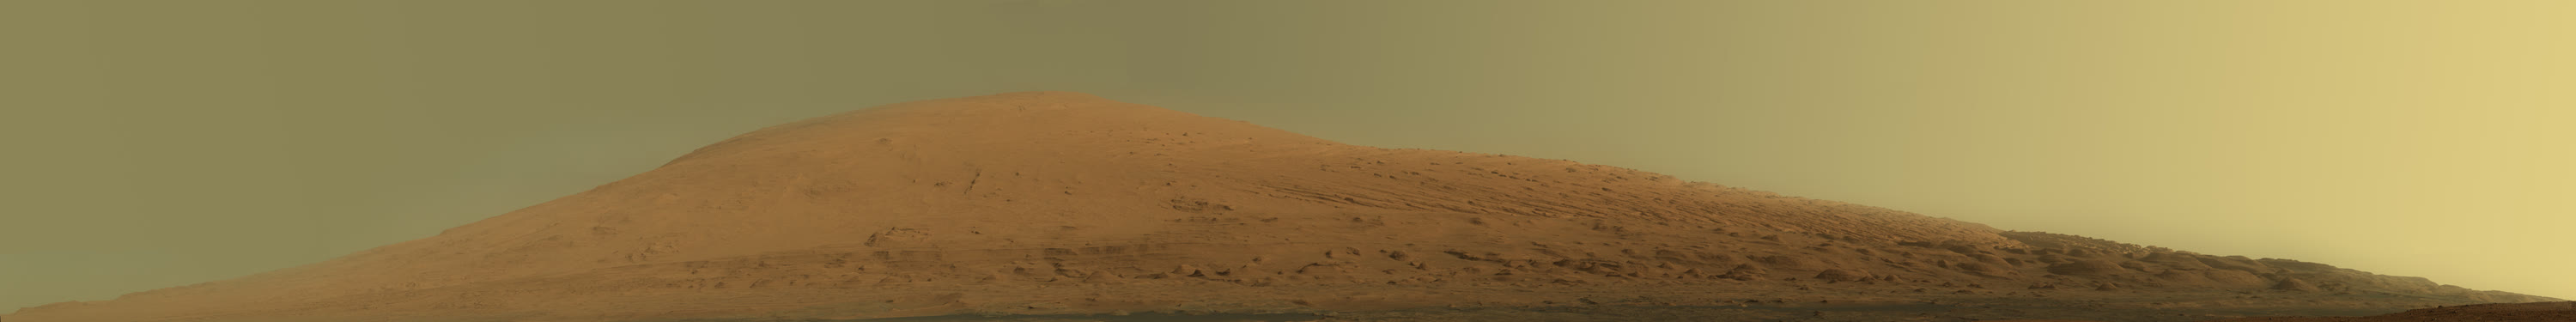
\includegraphics[width=0.96\linewidth]{images/book2/g10-nasa-mars-mount-sharp.jpg}

{\small Le mont Sharp, à l'intérieur du cratère Gale sur Mars, photographié
par le rover Curiosity en 2012, dans les couleurs enregistrées par sa
caméra. Ses couches inférieures se sont déposées dans l'eau, il y a des
milliards d'années. Image~: NASA/JPL-Caltech/MSSS (domaine public).}
\end{omfigure}

\section{La zone habitable}

\begin{definition}[Zone habitable]\label{def:g10:habitable-planet:habitable-zone}
La \emph{zone habitable}\index{zone habitable} d'une étoile est l'intervalle
de distances à l'étoile auquel une planète rocheuse pourvue d'assez d'eau et
d'une atmosphère semblable à celle de la Terre pourrait garder de l'eau
liquide à sa surface. Son bord intérieur est là où la planète perdrait son
eau sous l'effet de la chaleur~; son bord extérieur, là où même un fort effet
de serre ne pourrait plus l'empêcher de geler.
\end{definition}

\begin{proposition}[La zone habitable du Soleil]\label{prop:g10:habitable-planet:hz-sun}
% ledger: kopparapu:hz-sun, planet:Mercury.dist, planet:Venus.dist, planet:Mars.dist
Des modèles détaillés d'atmosphères planétaires placent la \omterm{def:g10:habitable-planet:habitable-zone}{zone habitable}
du Soleil entre \qty{0.99}{au} et \qty{1.70}{au}. La Terre (\qty{1}{au}) se
trouve juste à l'intérieur de son bord intérieur~; Mars (\qty{1.52}{au}) s'y
trouve aussi~; Vénus (\qty{0.72}{au}) se trouve nettement en deçà du bord
intérieur.
\end{proposition}

\begin{proposition}[Les zones habitables des autres étoiles]\label{prop:g10:habitable-planet:hz-scaling}
Autour d'une étoile de luminosité $L$, une planète reçoit le même
éclairement qu'à une distance $d_\odot$ du Soleil lorsqu'elle se trouve à
\[
  d = d_\odot \sqrt{L/L_\odot}.
\]
Les bords de la \omterm{def:g10:habitable-planet:habitable-zone}{zone habitable} se déplacent dans la même proportion, en
première approximation (la couleur de la lumière de l'étoile compte aussi
un peu).
\end{proposition}

\begin{proof}
Un éclairement égal signifie $L/(4\pi d^2) = L_\odot/(4\pi d_\odot^2)$,
donc $d^2 = d_\odot^2\,L/L_\odot$.
\end{proof}

\begin{omfigure}
\begin{tikzpicture}[font=\small]
  % top: the Sun, 0-2 au over 12 cm (6 cm per au)
  \fill[omProp!30] (0.99*6,0) rectangle (1.70*6,0.5);
  \draw[black!70] (0,0.25) -- (12.3,0.25);
  \foreach \x in {0,0.5,...,2} \draw (\x*6,0.15) -- (\x*6,0.35) node[pos=0, below=1pt, font=\footnotesize] {\x};
  \shade[ball color=yellow!70!orange] (0,0.25) circle (0.22);
  \foreach \n/\d in {Mercure/0.387, Vénus/0.723, Terre/1.0, Mars/1.524} {
    \fill[omThm!85!black] (\d*6,0.25) circle (2.2pt);
    \node[anchor=south, font=\footnotesize] at (\d*6,0.55) {\n};
  }
  \node[anchor=west, font=\footnotesize] at (12.4,0.25) {au};
  \node[anchor=north, font=\footnotesize] at (8.07,-0.25) {zone habitable, 0.99--1.70 au};
  \node[anchor=east, font=\footnotesize] at (-0.3,0.25) {Soleil};
  % bottom: Proxima Centauri, 0-0.1 au over 12 cm (120 cm per au)
  \begin{scope}[yshift=-2.2cm]
  \fill[omProp!30] (0.0385*120,0) rectangle (0.0661*120,0.5);
  \draw[black!70] (0,0.25) -- (12.3,0.25);
  \foreach \x/\l in {0/0, 0.025/0.025, 0.05/0.05, 0.075/0.075, 0.1/0.1} \draw (\x*120,0.15) -- (\x*120,0.35) node[pos=0, below=1pt, font=\footnotesize] {\l};
  \shade[ball color=red!70!orange] (0,0.25) circle (0.14);
  \fill[omThm!85!black] (0.0485*120,0.25) circle (2.2pt);
  \node[anchor=south, font=\footnotesize] at (0.0485*120,0.55) {Proxima b};
  \node[anchor=west, font=\footnotesize] at (12.4,0.25) {au};
  \node[anchor=north, font=\footnotesize] at (6.28,-0.25) {zone habitable, 0.038--0.066 au};
  \node[anchor=east, align=right, font=\footnotesize] at (-0.3,0.25) {Proxima\\du Centaure};
  \end{scope}
\end{tikzpicture}

{\small En haut~: la \omterm{def:g10:habitable-planet:habitable-zone}{zone habitable} du Soleil et les quatre planètes
rocheuses. En bas~: la \omterm{def:g10:habitable-planet:habitable-zone}{zone habitable} de la faible étoile rouge Proxima du
Centaure, calculée en multipliant celle du Soleil par la racine carrée de la
luminosité de l'étoile, et sa planète Proxima~b. Attention au changement
d'échelle~: toute la bande du bas mesure \qty{0.1}{au}.}
\end{omfigure}

\section{Les planètes des autres étoiles}

\begin{definition}[Exoplanète]\label{def:g10:habitable-planet:exoplanet}
Une \emph{exoplanète}\index{exoplanete@exoplanète} est une planète qui tourne
autour d'une autre étoile que le Soleil.
\end{definition}

Les \omterm{def:g10:habitable-planet:exoplanet}{exoplanètes} sont bien trop faibles et trop proches de leur étoile pour
être vues directement, à part quelques géantes. La plupart sont découvertes
indirectement~: soit la planète passe devant son étoile une fois par orbite
et en diminue très légèrement l'éclat, soit son attraction fait osciller
l'étoile vers nous puis en s'éloignant de nous, ce qui décale alternativement
la couleur de sa lumière. La seconde méthode ne donne qu'une masse
\emph{minimale} de la planète, car l'inclinaison de l'orbite n'est pas
connue. Ces méthodes sont étudiées dans le volume de 3\textsuperscript{e}~année.

\begin{dated}{2026}
% ledger: nea:count-2026
Le 15 octobre 2026, la NASA Exoplanet Archive recensait 6\,451 \omterm{def:g10:habitable-planet:exoplanet}{exoplanètes}
confirmées.
\end{dated}

\begin{example}[Proxima b]\label{ex:g10:habitable-planet:proxima}
% ledger: nea:proxima-b (flux and habitable zone computed in figdata/grade-10/planet_temperatures.py)
L'étoile la plus proche du Soleil, Proxima du Centaure, à
\qty{1.30}{\parsec}, est une petite étoile rouge dont la luminosité n'est
qu'environ $0.0015$ fois celle du Soleil. En 2016, on a découvert une
planète qui en fait le tour en 11.2 jours, à \qty{0.0485}{au}, avec au moins
1.06 fois la masse de la Terre. À cette distance, elle reçoit environ 0.64
fois l'éclairement que reçoit la Terre, et elle se trouve dans la \omterm{def:g10:habitable-planet:habitable-zone}{zone
habitable} de son étoile. On ne sait pas si elle a une atmosphère, ni de
l'eau.
\end{example}

\begin{remark}[Habitable ne veut pas dire habitée]\label{rem:g10:habitable-planet:inhabited}
La \omterm{def:g10:habitable-planet:habitable-zone}{zone habitable} n'énonce qu'une condition de distance et de lumière. Une
planète qui s'y trouve peut n'avoir ni eau ni atmosphère, ou pas la bonne
--- Mars se trouve dans la zone du Soleil et n'a pas d'eau liquide à sa
surface aujourd'hui. La Terre est habitable parce que plusieurs conditions
sont réunies à la fois~: la bonne distance, une masse assez grande pour
garder une atmosphère, de l'eau en abondance, et un effet de serre ni trop
faible ni trop fort.
\end{remark}

\section{Exercices}

\begin{exercise}[$\star$]\label{exo:g10:habitable-planet:1}
Définir la \omterm{def:g10:habitable-planet:equilibrium-temperature}{température d'équilibre} d'une planète. Pourquoi la température
moyenne de la surface de la Terre est-elle supérieure à sa \omterm{def:g10:habitable-planet:equilibrium-temperature}{température
d'équilibre}~?
\end{exercise}

\begin{exercise}[$\star$]\label{exo:g10:habitable-planet:2}
À l'aide du diagramme en barres des \omterm{def:g10:habitable-planet:equilibrium-temperature}{températures d'équilibre} et mesurées,
nommer le corps dont la surface est le plus réchauffée par son atmosphère,
et estimer de combien de kelvins.
\end{exercise}

\begin{exercise}[$\star$]\label{exo:g10:habitable-planet:3}
Mars tourne à \qty{1.52}{au} du Soleil. À l'aide de la loi en inverse du
carré, avec $S_0 = \qty{1361}{W/m^2}$, calculer l'éclairement solaire sur
Mars.
\end{exercise}

\begin{exercise}[$\star$]\label{exo:g10:habitable-planet:4}
À l'aide du diagramme de phases de l'eau, donner l'état de l'eau à
\qty{1}{bar} et \qty{330}{K}~; à \qty{0.001}{bar} et \qty{250}{K}~; à
\qty{100}{bar} et \qty{700}{K}.
\end{exercise}

\begin{exercise}[$\star$]\label{exo:g10:habitable-planet:5}
Qu'est-ce qu'une \omterm{def:g10:habitable-planet:exoplanet}{exoplanète}~? Décrire, en une phrase chacune, les deux
principales méthodes de détection des \omterm{def:g10:habitable-planet:exoplanet}{exoplanètes}.
\end{exercise}

\begin{exercise}[$\star\star$]\label{exo:g10:habitable-planet:6}
Calculer la \omterm{def:g10:habitable-planet:equilibrium-temperature}{température d'équilibre} de la Terre avec
$S_0 = \qty{1361}{W/m^2}$ et $A = 0.294$, puis avec $A = 0$. Convertir les
deux résultats en degrés Celsius.
\end{exercise}

\begin{exercise}[$\star\star$]\label{exo:g10:habitable-planet:7}
Une étoile est quatre fois plus lumineuse que le Soleil. Entre quelles
distances se situe sa \omterm{def:g10:habitable-planet:habitable-zone}{zone habitable}~? La Terre, placée à \qty{1}{au} de
cette étoile, s'y trouverait-elle~?
\end{exercise}

\begin{exercise}[$\star\star$]\label{exo:g10:habitable-planet:8}
Vénus tourne à \qty{0.723}{au}. Calculer l'éclairement qu'elle reçoit, puis
sa \omterm{def:g10:habitable-planet:equilibrium-temperature}{température d'équilibre} avec son albédo de Bond de 0.77. Comparer à sa
température de surface de \qty{737}{K} et expliquer l'écart.
\end{exercise}

\begin{exercise}[$\star\star$]\label{exo:g10:habitable-planet:9}
Sur Mars, la pression moyenne en surface est de \qty{6.36}{mbar}, juste
au-dessus du point triple de l'eau, et l'eau y bout vers
\qty{0.5}{\degreeCelsius}. Expliquer pourquoi l'eau liquide ne peut pas
subsister à la surface de Mars aujourd'hui, même par un après-midi d'été où
le sol atteint \qty{10}{\degreeCelsius}.
\end{exercise}

\begin{exercise}[$\star\star$]\label{exo:g10:habitable-planet:10}
La vitesse de libération vaut \qty{2.4}{km/s} sur la Lune et
\qty{11.2}{km/s} sur la Terre. Calculer leur rapport. Expliquer pourquoi la
Terre a gardé une atmosphère et la Lune non.
\end{exercise}

\begin{exercise}[$\star\star$]\label{exo:g10:habitable-planet:11}
Supposons que la Terre soit couverte de glace et que son albédo de Bond
monte à 0.50. Calculer sa nouvelle \omterm{def:g10:habitable-planet:equilibrium-temperature}{température d'équilibre}. Expliquer
pourquoi un tel état, une fois atteint, tendrait à durer.
\end{exercise}

\begin{exercise}[$\star\star\star$]\label{exo:g10:habitable-planet:12}
Montrer que $T_{\mathrm{eq}} = \qty{278.3}{K} \times (1-A)^{1/4}/\sqrt{d}$,
avec $d$ en unités astronomiques, découle de la formule du chapitre. Par
quel facteur la \omterm{def:g10:habitable-planet:equilibrium-temperature}{température d'équilibre} est-elle multipliée quand la
distance est multipliée par quatre~?
\end{exercise}

\begin{exercise}[$\star\star\star$]\label{exo:g10:habitable-planet:13}
À quelle distance du Soleil une planète d'albédo 0.294 aurait-elle une
\omterm{def:g10:habitable-planet:equilibrium-temperature}{température d'équilibre} de \qty{273}{K}~? Comparer au bord intérieur de la
\omterm{def:g10:habitable-planet:habitable-zone}{zone habitable}, et expliquer pourquoi les deux diffèrent.
\end{exercise}

\begin{exercise}[$\star\star\star$]\label{exo:g10:habitable-planet:14}
Sur une planète dont la pression en surface est de \qty{1000}{Pa}, l'eau
bout vers \qty{7}{\degreeCelsius}. Entre quelles températures l'eau
peut-elle y être liquide~? Que deviendrait un lac de cette planète par une
journée à \qty{15}{\degreeCelsius}~?
\end{exercise}

\begin{exercise}[$\star\star\star$]\label{exo:g10:habitable-planet:15}
Une planète tourne à \qty{1.2}{au} d'une étoile deux fois moins lumineuse
que le Soleil. Calculer les bords de la \omterm{def:g10:habitable-planet:habitable-zone}{zone habitable} de l'étoile et dire
si la planète s'y trouve. Quelle confiance peut-on accorder à la réponse~?
\end{exercise}

\section{Problème~: Proxima~b pourrait-elle porter un océan~?}

\begin{problem}[{Problème du week-end --- de la lumière d'une faible étoile
rouge à la température de sa planète la plus proche}]
\label{pb:g10:habitable-planet:1}
% ledger: nea:proxima-b, kopparapu:hz-sun, earth:TSI, earth:albedo, planet:Earth.vesc, nasa:bond-albedos (all results computed in figdata/grade-10/planet_temperatures.py or from the rounded data below)
Une élève lit la fiche de données de la planète Proxima~b. Son étoile a une
luminosité $L = 0.00151\,L_\odot$~; la planète tourne à
$d = \qty{0.0485}{au}$ en 11.18 jours et a au moins 1.055 fois la masse de
la Terre. On utilisera $S_0 = \qty{1361}{W/m^2}$,
$\sigma = \qty{5.67e-8}{W.m^{-2}.K^{-4}}$, la \omterm{def:g10:habitable-planet:habitable-zone}{zone habitable} du Soleil
\qtyrange{0.99}{1.70}{au}, et la vitesse de libération de la Terre
\qty{11.2}{km/s}.

\medskip
\noindent\textbf{Partie I --- La lumière de l'étoile.}
\begin{enumerate}
  \item Calculer l'éclairement reçu par la planète en fraction de celui de
        la Terre, $L/d^2$ (avec $L$ en luminosités solaires et $d$ en au).
  \item L'exprimer en \unit{W/m^2}.
  \item Le comparer à l'éclairement sur Vénus (\qty{2601}{W/m^2}) et sur
        Mars (\qty{586}{W/m^2}).
  \item Combien d'années de la planète tiennent dans une année terrestre~?
\end{enumerate}

\medskip
\noindent\textbf{Partie II --- Des températures sans atmosphère.}
\begin{enumerate}[resume]
  \item Calculer la \omterm{def:g10:habitable-planet:equilibrium-temperature}{température d'équilibre} d'une planète parfaitement
        sombre ($A = 0$) sous cet éclairement.
  \item La calculer pour une planète aussi brillante que Vénus
        ($A = 0.77$).
  \item Laquelle de ces deux températures dépasse le point de congélation
        de l'eau~? Que montrent les deux résultats sur le rôle des nuages et
        de la glace~?
\end{enumerate}

\medskip
\noindent\textbf{Partie III --- La zone habitable.}
\begin{enumerate}[resume]
  \item Calculer $\sqrt{L/L_\odot}$.
  \item Calculer le bord intérieur de la \omterm{def:g10:habitable-planet:habitable-zone}{zone habitable} de l'étoile.
  \item Calculer son bord extérieur.
  \item Proxima~b se trouve-t-elle dans la \omterm{def:g10:habitable-planet:habitable-zone}{zone habitable}~?
  \item À quelle distance du Soleil une planète recevrait-elle le même
        éclairement que Proxima~b~? Où cela se situerait-il dans la \omterm{def:g10:habitable-planet:habitable-zone}{zone
        habitable} du Soleil~?
\end{enumerate}

\medskip
\noindent\textbf{Partie IV --- Une atmosphère et de l'eau~?}
\begin{enumerate}[resume]
  \item Si la planète avait la masse volumique moyenne de la Terre, son
        rayon serait $1.055^{1/3}$ fois celui de la Terre. Calculer ce
        facteur.
  \item La vitesse de libération est proportionnelle à $\sqrt{M/R}$.
        Estimer la vitesse de libération de la planète. Pourrait-elle garder
        une atmosphère~?
  \item Pourquoi ne connaît-on qu'une valeur minimale de la masse~?
  \item Sur le diagramme de phases, quelle est la plus faible pression en
        surface qui permettrait l'existence d'eau liquide~?
  \item Calculer la \omterm{def:g10:habitable-planet:equilibrium-temperature}{température d'équilibre} de Proxima~b avec l'albédo de
        la Terre, 0.294.
  \item De combien de kelvins son effet de serre devrait-il alors la
        réchauffer pour amener sa surface à la température moyenne de la
        Terre, \qty{288}{K}~?
\end{enumerate}
\end{problem}
